\noindent
\begin{tabular}{cc}
\begin{minipage}[c]{0.60\textwidth}
\begin{exerciseS}[Corrente libera su parete inclinata]
Si consideri una corrente d'acqua a pelo libero, laminare e stazionaria, che
scorre su una parete piana di lunghezza e apertura infinita  inclinata di un angolo $\alpha$ rispetto all'orizzontale.
Sul pelo libero la pressione è uniforme e uguale a $P_a$. Lo sforzo tangenziale fra acqua e aria viene considerato nullo.

Si calcoli il profilo di velocità nello strato di acqua e il campo di pressione.
\end{exerciseS}
\end{minipage}
\begin{minipage}[c]{0.35\textwidth}
   \begin{center}
   \includegraphics[width=0.90\textwidth]{./fig/slnEsatte-scivolo}
   \end{center}
\end{minipage}
\end{tabular}

\sol

\partone
 Semplificazione delle equazioni di NS in casi particolari. 
Soluzioni esatte in coordinate cartesiane.

\parttwo
Si scelga un sistema di riferimento cartesiano con l'asse $x$ orientato lungo la parete verso il basso e l'asse y perpendicolare ed uscente ad essa.
Sulla corrente di questo problema agiscono le forze di volume dovute alla gravità.
L'ipotesi che la pressione sia uniforme sulla superficie di interfaccia
 tra acqua e aria implica che la pressione è indipendente dalla coordinata $x$ in tutto il fluido.
% : si dimostra che $\dfrac{\partial p}{\partial y}=0$; se sulla superficie libera la pressione è costante e non varia nello spessore, allora la pressione è costante in tutto il fluido.

\begin{itemize}

   \item Scrittura delle equazioni di NS in coordinate cartesiane in 2 dimensioni.
%  
 \begin{equation}
\begin{cases}
  \dfrac{\partial u}{\partial t} + u \dfrac{\partial u}{\partial x}
  + v \dfrac{\partial u}{\partial y} - \nu \left( 
  \dfrac{\partial^2 u}{\partial x^2} +
  \dfrac{\partial^2 u}{\partial y^2} \right)
  + \dfrac{1}{\rho} \dfrac{\partial p}{\partial x} = f_x \\
  \dfrac{\partial v}{\partial t} + u \dfrac{\partial v}{\partial x}
  + v \dfrac{\partial v}{\partial y} - \nu \left( 
  \dfrac{\partial^2 v}{\partial x^2} +
  \dfrac{\partial^2 v}{\partial y^2} \right)
  + \dfrac{1}{\rho} \dfrac{\partial p}{\partial y} = f_y \\
  \dfrac{\partial u}{\partial x} + \dfrac{\partial v}{\partial y} = 0
\end{cases}
\end{equation}

  \item Semplificazione delle equazioni di NS per il problema considerato. Vengono fatte le seguenti ipotesi:
\begin{itemize}
\item problema stazionario: $\dfrac{\partial}{\partial t} = 0$;
\item direzione $x$ omogenea (canale infinito in direzione $x$): $\dfrac{\partial u}{\partial x} = \dfrac{\partial v}{\partial x} = 0$; 
\begin{remark}
non si può dire altrettanto della pressione, a causa del ruolo che questa ha nelle equazioni di NS incomprimibili. Il campo di pressione può essere interpretato come un moltiplicatore di Lagrange necessario a imporre il vincolo di incomprimibilità. Inoltre, ad eccezione di alcune condizioni al contorno, non appare mai direttamente come pressione $p$ ma solamente con le sue derivate spaziali. Da un punto di vista più fisico, la differenza di pressione lungo il canale è la forzante che mette in moto il fluido in una corrente di Poiseuille.
\end{remark}
\item la condizione $\dfrac{\partial u}{\partial x} = 0$ inserita nel vincolo di incomprimibilità, implica $\dfrac{\partial v}{\partial y}=0$; poichè $\dfrac{\partial v}{\partial x}=\dfrac{\partial v}{\partial y}=0$ segue che $v = \text{cost} = 0$, poiché è nulla a parete per la condizione al contorno di adesione, $\bm{u} = \bm{0}$.
\item no forze di volume: $\bm{f} = \rho \bm{g} = \rho g \sin \alpha \bm{\hat{x}} - \rho g \cos \alpha \bm{\hat{y}}$.
\end{itemize}
%
Le equazioni di NS possono essere semplificate 
\begin{equation}
\begin{cases}
  - \mu \dfrac{\partial^2 u}{\partial y^2} = - \dfrac{\partial p}{\partial x} + \rho g \sin \alpha \\
  \dfrac{\partial p}{\partial y} = - \rho g \cos \alpha \ .
\end{cases}
\end{equation}

Dalla seconda segue che l'espressione del campo di pressione è
\begin{equation}
 p(x,y) = -\rho g y \cos \alpha + f(x) \ .
\end{equation}
L'espressione di $f(x)$ può essere calcolata imponendo la condizione al contorno sul pelo libero, $p(x,H) = P_a$,
\begin{equation}
 P_a = -\rho g H \cos \alpha + f(x) \qquad \rightarrow \qquad f(x) = P_a + \rho g H \cos \alpha \ .
\end{equation}
La funzione $f(x)$ è costante, senza dipendere dalla coordinata $x$. Di conseguenza, il campo di pressione dipende solo dalla coordinata $y$
\begin{equation}
 p(x,y) = P_a + \rho g ( H - y ) \cos \alpha \ ,
\end{equation}
e la derivata di $\partial p / \partial x$ è nulla. La componente $x$ dell'equazione della quantità di moto diventa quindi un'equazione ordinaria del secondo ordine
\begin{equation}
   \begin{cases}
    - \mu u''(y) = \rho g  \sin \alpha  \ , \ y \in[0,H] \\
    u(0) = 0  \\ u'(H) = 0 \ ,
  \end{cases}
\end{equation}
con le condizioni al contorno di adesione a parete e di sforzo di taglio nullo all'interfaccia tra aria ed acqua, $0=\tau(H)=\mu \dfrac{\partial u}{\partial y}(H)=\mu u'(H)$. La derivata parziale in $y$ è stata sostituita da quella ordinaria, poichè
 la velocità è solo funzione di $y$.
  
  \item Soluzione dell'equazione differenziale  con dati al contorno: si integra due volte e si impongono le condizioni al contorno per ottenere la componente $u$ del campo di velocità.
  \begin{equation}
   u(y) = - \dfrac{\rho g}{2 \mu} y( y - H ) \sin \alpha \ .
  \end{equation}
  
\end{itemize}

